\documentclass[11pt]{article}
\usepackage{graphicx}
\usepackage{amssymb}
\usepackage{epstopdf}
\usepackage{latexsym}
\usepackage{amsmath}
\usepackage{mathdots}
\usepackage{float}
\usepackage[dvips,letterpaper,margin=1 in]{geometry}
%\DeclareGraphicsRule{.tif}{png}{.png}{`convert #1 `dirname #1`/`basename #1 .tif`.png}


\title{}
\author{}
\date{}
\newtheorem{pb}{Paper}
\newcommand{\tr}{\mbox{tr}}

%Begin Problem 1
\begin{document}
\begin{flushleft}
\textbf{\Large{CS 244 Project Proposal}}
\begin{flushright} Spring '16, Sean Choi, Eyal Cidon
\end{flushright}
\end{flushleft}

\begin{pb}
Abstractions for Network Update
\end{pb}
One of the paper that we would like to replicate is the paper on the abstraction on network updates. The paper discusses the fundamental problem of difficulties in updating the network states. The author points out the following facts. Even with the arrival of SDN that hugely simplified the management of network configurations, the changes are still very low level and very prone to errors. Also, there are network states that cannot be exhaustively considered due to the complexity and the size of the network, such as considering a packet in flight at a given point in time.

In order to solve this, the authors provide an abstraction to provide an high-level abstraction that allow the programmers to simply update the configuration of the entire network. The primary abstraction is that each packets and the packets within the same flow must be processed by a single global network configuration. Given such abstractions, the authors provide several update mechanisms using the features in OpenFlow to support it. Then the author provides a theoretical model that the abstractions have been correctly implemented, as well as a verification tool to verify the properties. 

The main result we would like to see is something like the following graph.
\begin{figure}[H]
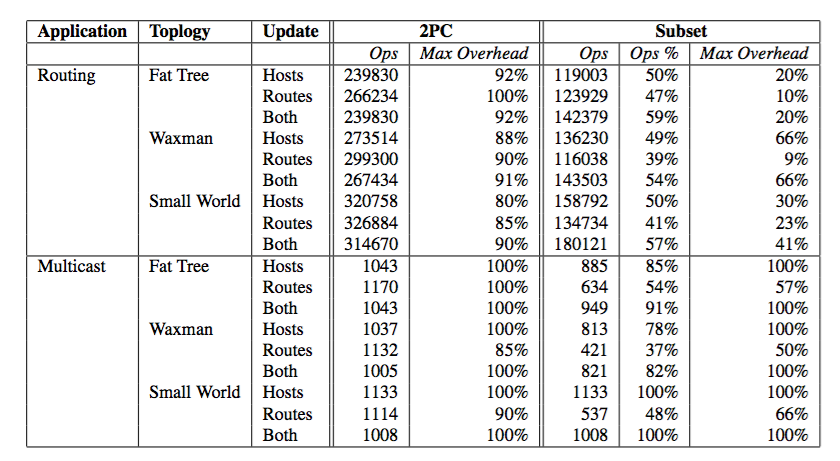
\includegraphics[width=16cm]{table}
\centering
\end{figure}

This table represents the comparison between the number of Openflow install operations between a two-phase update and Subset (the optimization in this paper). This experiment was run on Mininet topology. We hope to replicate the similar experiment as follows. First we would set up a Mininet topology and come up with upgrade plans for routing that will be mapped to both 2PC and Subset. Then, we will compare the number of operations on OpenFlow just as this table. We hope to see a similar reduction in number of operations.

\newpage
\begin{pb}

\end{pb}
\end{document}